% !TEX program = xelatex
\documentclass[UTF8,fontset=mac,11pt,letterpaper]{ctexart}
\usepackage[textwidth=6.55in,textheight=9.1in,top=.85in]{geometry}
\usepackage{pifont}
\usepackage{fontspec,newtxmath,amsmath,graphicx,booktabs,array,longtable,multirow}
\usepackage[numbers,square,sort&compress]{natbib}
\usepackage{xurl,hyperref,caption,fancyhdr,microtype,setspace}
\usepackage{placeins}
\usepackage{float}
\setmainfont{texgyretermes-regular.otf}[BoldFont=texgyretermes-bold.otf,ItalicFont=texgyretermes-italic.otf,BoldItalicFont=texgyretermes-bolditalic.otf]
\hypersetup{colorlinks=true,linkcolor=black,citecolor=black,urlcolor=black,pdftitle={从分词器到 PDE 发现}}
\captionsetup{font=small,labelfont=bf,labelsep=quad,skip=5pt}
\setlength{\parindent}{1em}\setlength{\parskip}{2pt}\setstretch{1.05}
\setlength{\textfloatsep}{12pt}\setlength{\floatsep}{10pt}\setlength{\intextsep}{10pt}
\setlength{\emergencystretch}{1.5em}\setlength{\tabcolsep}{4pt}\renewcommand{\arraystretch}{1.15}
\ctexset{section={format=\large\bfseries,beforeskip=13pt,afterskip=6pt},subsection={format=\normalsize\bfseries,beforeskip=9pt,afterskip=4pt}}
\pagestyle{fancy}\fancyhf{}\fancyfoot[C]{\small\thepage}\setlength{\headheight}{13pt}\setlength{\headsep}{18.9pt}\addtolength{\topmargin}{6.1pt}\setlength{\footskip}{38pt}\renewcommand{\headrulewidth}{0pt}
\title{从分词器到 PDE 发现}\author{}\date{}
\makeatletter\renewcommand{\maketitle}{\begin{center}{\LARGE\bfseries\@title\par}\end{center}\vspace{8pt}}\makeatother
\newcommand{\fig}[3]{\begin{figure}[!htbp]\centering\includegraphics[width=#2\linewidth]{figures/#1.pdf}\caption{#3}\label{fig:#1}\end{figure}}
\begin{document}
\maketitle\thispagestyle{fancy}
\section{背景}
\subsection{前置知识}
\paragraph{EqGPT。}
EqGPT从数学手册收集PDE，将基本项与运算符编码为方程生成式表示（generative representation of equations，GRE），并训练自回归Transformer预测下一个token。与之并行，观测数据用于训练场的代理网络；该网络重建观测场，通过自动微分计算导数，为候选方程提供数值评价数据。

发现阶段采用“生成—评价—微调”循环：模型从起始符逐步采样，直至生成完整方程结构；随后在代理网络提供的数据上以最小二乘拟合系数，结合拟合优度与项数计算评分；评分最高的十个候选用于监督微调（SFT），再由更新后的模型生成下一轮候选。循环结束后选出最高分结构，并进一步优化系数。

\begin{figure}[H]
\centering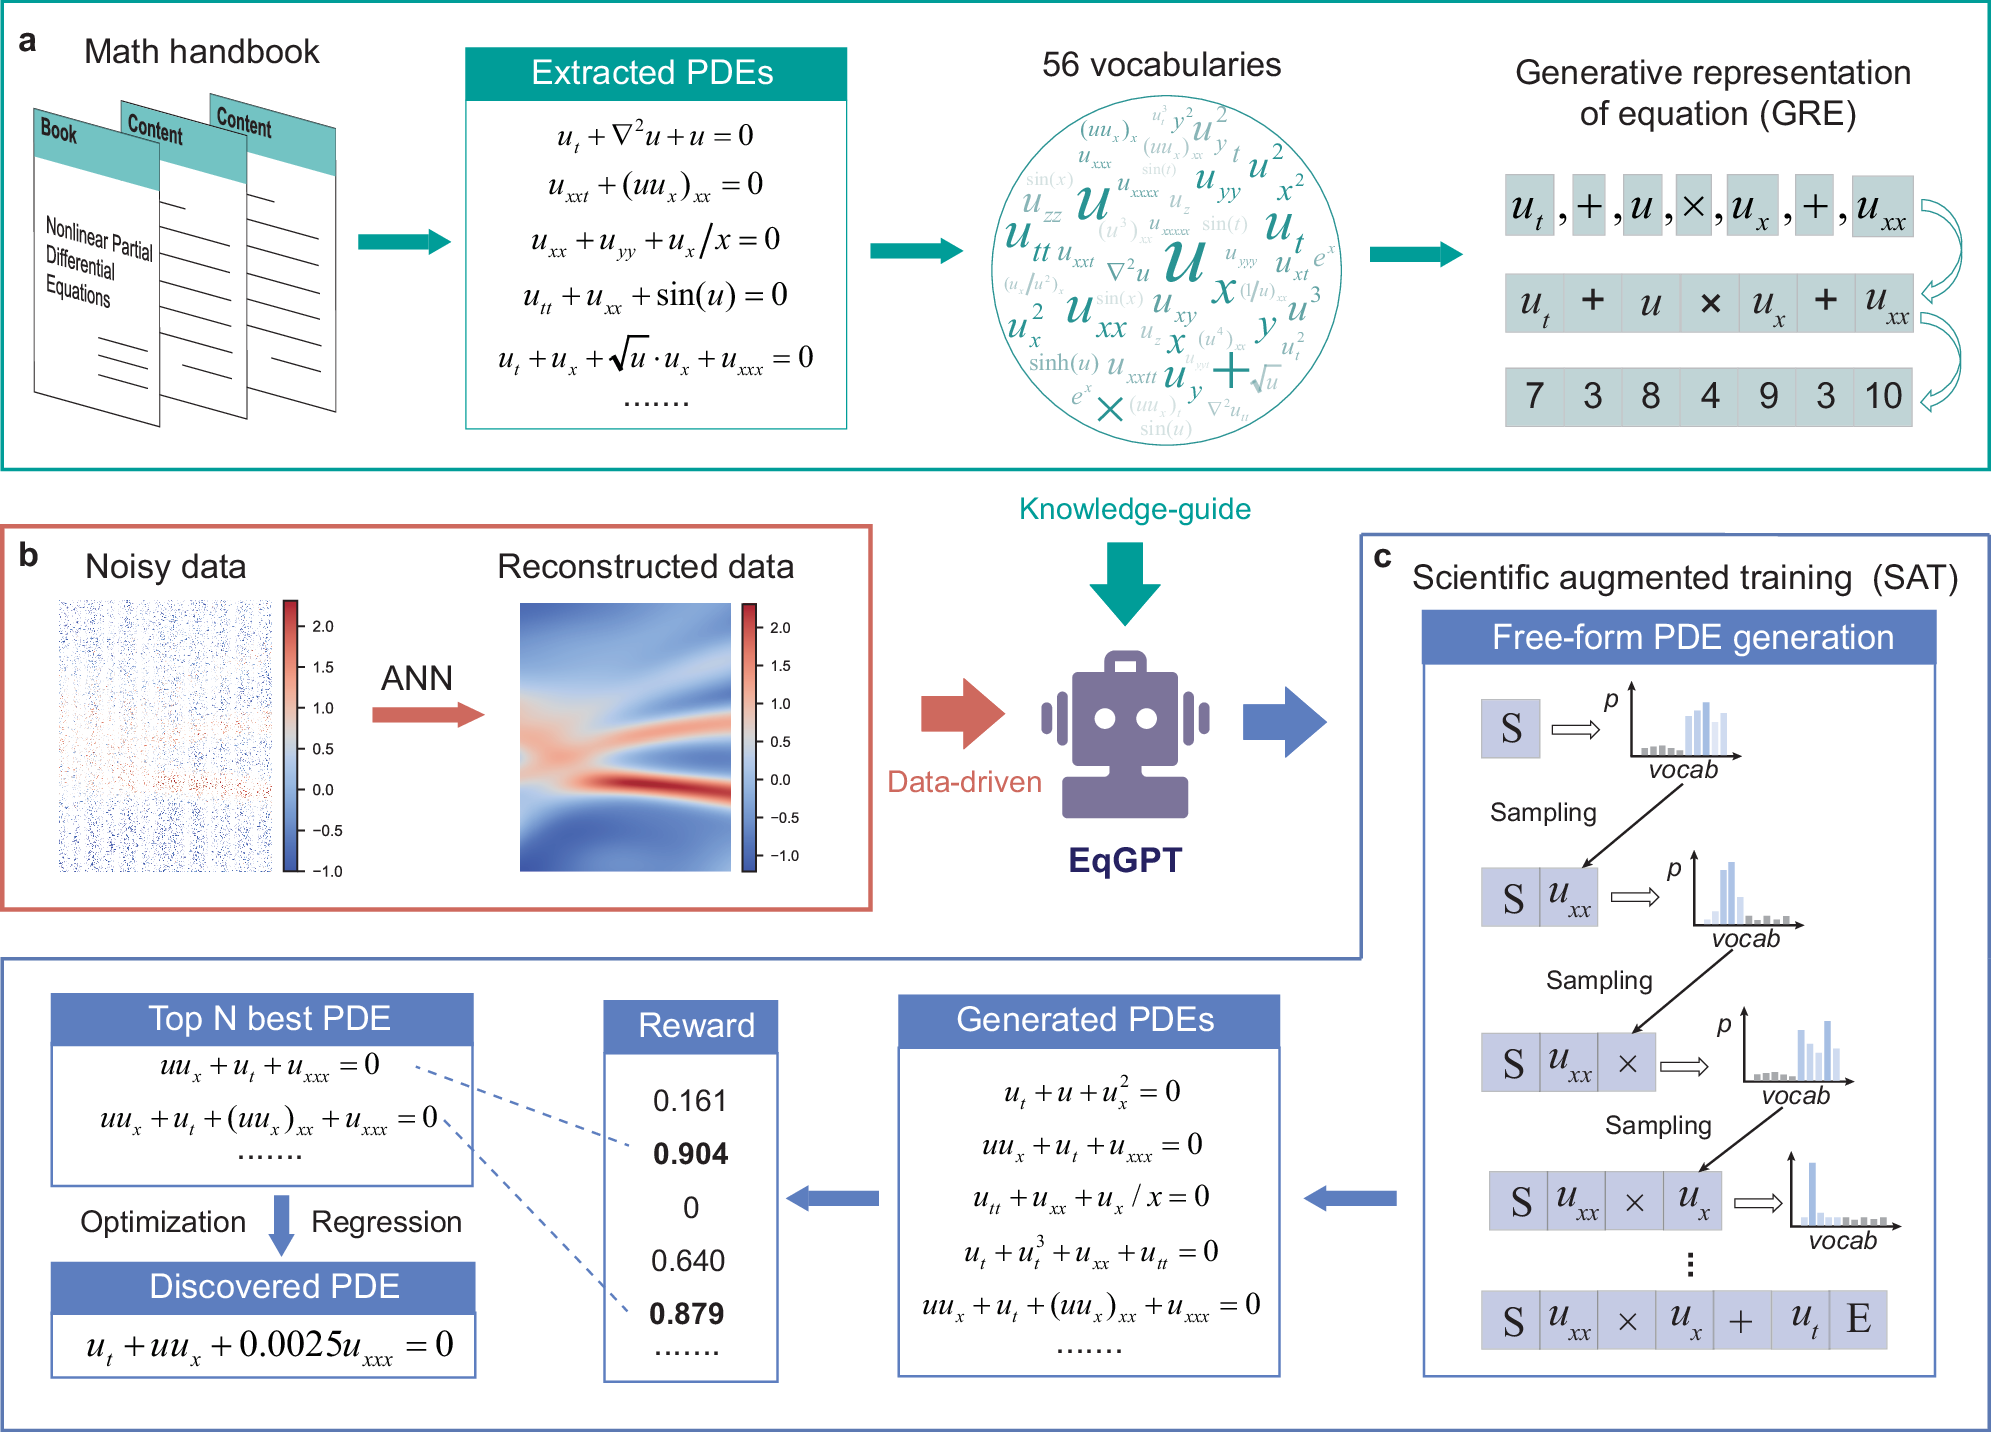
\includegraphics[width=\linewidth]{figures/eqgpt_original.png}
\caption*{\textbf{EqGPT原论文流程示意图。}}
\end{figure}

\subsection{与EqGPT的差别}\label{subsec:changes}
本文在EqGPT框架中采用两项修改。

\textbf{更换分词器。}原始EqGPT直接编码GRE基本项与运算符；本文使用AST-BPE作为分词器。词表使用未增强的语料训练，Transformer使用增强语料训练。

\begin{samepage}
\textbf{取消生成时的SAT语法约束。}AST-BPE模型直接按token概率生成LaTeX，不使用EqGPT里的SAT（即利用人工规则确保模型输出合法PDE）。
\end{samepage}

\section{实验设置}
\subsection{八个PDE案例}
我们使用表\ref{tab:cases}中的八个单场PDE案例，观察模型能不能从数据里发现对应的目标方程。

\begin{table}[!htbp]
\caption{八个目标方程。$u=u(x,t)$，下标表示偏导数；PDE-divide在$x\ne0$的区域评价。}\label{tab:cases}
\centering\small
\begin{tabular*}{\linewidth}{@{\extracolsep{\fill}}ll@{}}\toprule
案例 & 目标方程\\\midrule
Wave & $u_{tt}-u_{xx}=0$\\
Convection--diffusion & $u_t+u_x-0.25u_{xx}=0$\\
Klein--Gordon & $u_{tt}-0.5u_{xx}+5u=0$\\
Burgers & $u_t+uu_x-0.1u_{xx}=0$\\
Eq.\ 6.2.12 & $u_t+0.1u_{xt}+0.1u_x=0$\\
PDE-divide & $u_t+u_x/x+0.25u_{xx}=0$\\
KdV & $u_t+uu_x+0.0025u_{xxx}=0$\\
Chaffee--Infante & $u_t-u_{xx}+u-u^3=0$\\\bottomrule
\end{tabular*}
\end{table}

\subsection{训练语料与划分}
语料分为小语料和大语料，分别包含212条和636条方程。大语料在小语料的基础上增加424条方程，新增方程涵盖输运、反应--扩散、波动、椭圆、色散和高阶PDE。

上下游任务使用相同的大语料，实际划分见表\ref{tab:splits}。
\begin{table}[H]
\caption{上下游任务的语料划分。下游测试为表\ref{tab:cases}的八个PDE案例，不另设语料测试集。}\label{tab:splits}
\centering\small
\begin{tabular*}{\linewidth}{@{\extracolsep{\fill}}llrrrr@{}}\toprule
任务 & 语料 & 总数 & 训练 & 验证 & 测试\\\midrule
上游分词 & 大语料 & 636 & 509 & 64 & 63\\
下游发现 & 小语料 & 212 & 191 & 21 & --\\
下游发现 & 大语料 & 636 & 572 & 64 & --\\\bottomrule
\end{tabular*}
\end{table}

\subsection{训练与搜索参数}
各模型使用六层Transformer。预训练采用余弦退火与验证集早停，最长200个epoch。每次PDE发现进行五轮搜索，每轮获得400个成功评分候选，再用高分候选进行五个epoch的SFT。正文主实验中的所有模型均采用80\%按模型分布采样、20\%随机采样，与原始EqGPT的配置一致。随机采样对发现结果的影响较大，具体对照结果见附录\ref{app:sampling}。

实验运行525、526和527三个种子\footnote{正文所有实验结果均选取种子525。}完整参数及其他种子结果见附录\ref{app:params}与\ref{app:seeds}。

\subsection{评估指标}
\paragraph{分词表现。}
\begin{itemize}\setlength{\itemsep}{2pt}\setlength{\parsep}{0pt}
\item \textbf{压缩率。}$C=N_{\rm initial}/N_{\rm final}$，即使用初始词表获得的token数量除以使用最终词表获得的token数量。
\item \textbf{命令完整率。}$I_{\rm cmd}$为完整LaTeX命令内部没有被切开的比例。
\item \textbf{数字完整率。}$I_{\rm num}$为完整数字串内部没有被切开的比例。
\item \textbf{词表使用率。}新增token指BPE通过合并得到的token，不包括初始字符和控制符。定义为
\begin{equation}
 U=\frac{\text{实际用到的新增token种数}}{\text{新增token总种数}}.
\end{equation}
例如，词表新增了\verb|u_t|、\verb|u_x|、\verb|u_{xx}|、\verb|\sin|和\verb|\cos|五种token；若验证集的最终编码只用到前两种，则$U=2/5=40\%$。同一种token无论出现多少次，都只计一种。该指标反映新增token在评价数据中的使用范围。

\end{itemize}

\paragraph{PDE发现。}
结构相同指不考虑系数时，公式结构相同。
\begin{itemize}\setlength{\itemsep}{2pt}\setlength{\parsep}{0pt}
\item \textbf{Top1。}最终reward最高的候选公式是否与目标方程结构相同。
\item \textbf{Top10。}最终reward最高的十个候选公式中是否存在与目标方程结构相同的公式。
\item \textbf{Reward。}数值评分沿用EqGPT：
\begin{equation}\label{eq:reward}
 r=\left(1-0.2\log_{10}M\right)R^2.
\end{equation}
\end{itemize}

\section{实验与结果}
\subsection{上游任务}
在上游任务中，我们进行了三个实验，分别研究各类分词器的性能、词表大小对AST-BPE的影响以及分词器的泛化能力。

首先，我们评估了各类分词器在636条语料上的表现（见表\ref{tab:upstream}）。按照表\ref{tab:splits}划分数据，仅用训练集学习AST-BPE词表，再将AST-BPE与Qwen2.5、Llama 3和\texttt{o200k\_base}用于同一测试集，计算分词指标。可以看到，词表大小为300和450时均保持了完整LaTeX命令，压缩率分别为6.983和8.497，三个通用分词器为1.725--1.796。通用分词器的命令完整率为零，这说明反斜杠与命令名之间存在切分。

\begin{table}[!htbp]
\caption{基于636条语料的上游测试结果。}\label{tab:upstream}
\centering\small\begin{tabular*}{\linewidth}{@{\extracolsep{\fill}}lrrrr@{}}\toprule
分词器 & 压缩率$\uparrow$ & 命令完整率(\%) & 数字完整率(\%) & 使用率(\%)\\\midrule
AST-BPE 300 & 6.983 & \textbf{100.0} & 100.0 & 35.7\\
AST-BPE 450 & \textbf{8.497} & \textbf{100.0} & 100.0 & 26.2\\
Qwen2.5 & 1.796 & 0.0 & 100.0 & --\\
Llama 3 & 1.796 & 0.0 & 100.0 & --\\
\texttt{o200k\_base} & 1.725 & 0.0 & 100.0 & --\\
\bottomrule\end{tabular*}
\end{table}



此外，我们还分析了词表大小对压缩率和使用率的影响（见图\ref{fig:capacity_tradeoff}）。我们在相同的上游任务数据集上，将AST-BPE词表大小设为100、120、150、200、250、256、300、350、400、450、500和512，评估其压缩率和使用率。可以发现，词表增大时，压缩率上升，词表使用率下降。词表大小从300增至450时，验证集压缩率由7.235升至8.967，使用率由38.4\%降至29.4\%。

\begin{figure}[H]\centering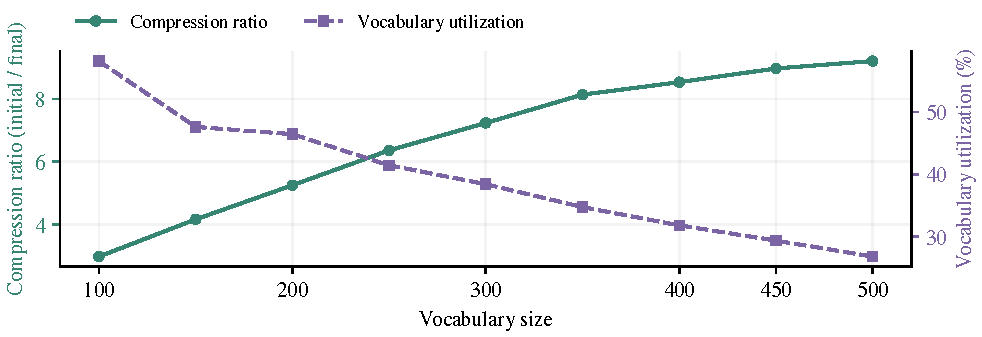
\includegraphics[width=\linewidth]{figures/capacity_tradeoff.pdf}\caption{验证集上不同词表大小对应的压缩率与词表使用率。}\label{fig:capacity_tradeoff}\end{figure}

此外，我们还评估了分词器的泛化能力。我们利用相对简单的公式训练分词器，并在复杂公式上测试它。具体的泛化实验见附录\ref{app:generalization}。


\FloatBarrier
\subsection{下游任务}
我们评估了分词器对模型PDE发现能力的影响。我们对EqGPT进行两项修改（见第\ref{subsec:changes}节），分别用小语料和大语料对EqGPT与修改后的AST-BPE EqGPT进行预训练，最后在八个测试案例上观察模型能否从数据中发现对应的目标PDE（见表\ref{tab:main}）。

可以看到，两档语料下AST-BPE EqGPT整体表现更好：小语料下，词表大小为300和450的模型分别发现6个和7个正确结构，高于EqGPT的3个；大语料下，分别为3个和2个，EqGPT为2个。与小语料相比，大语料下三种模型的成功案例数均减少，这一现象将在第四部分仔细分析。

\begin{table}[H]
\caption[八案例发现结果]{八案例发现结果\protect\footnotemark。表中逐一列出八个案例的结果；每格前一项为Top1是否正确，后一项为Top10是否包含正确结构。\ding{51}表示成功，\ding{55}表示未成功。CD为对流--扩散，KG为Klein--Gordon，E6为Eq.\ 6.2.12，PD为PDE-divide，CI为Chaffee--Infante。总计列为两类成功案例数，组内最高值加粗。}\label{tab:main}
\centering\fontsize{8.5}{10}\selectfont\setlength{\tabcolsep}{2pt}\begin{tabular*}{\linewidth}{@{\extracolsep{\fill}}llccccccccr@{}}
\toprule
语料 & 模型 & Wave & CD & KG & Burgers & E6 & PD & KdV & CI & 总计\\
\midrule
212 & EqGPT & \ding{51}/\ding{51} & --/\ding{51} & --/\ding{51} & --/\ding{51} & --/-- & --/\ding{51} & \ding{51}/\ding{51} & \ding{51}/\ding{51} & 3/\textbf{7}\\
 & AST-BPE 300 & \ding{51}/\ding{51} & \ding{51}/\ding{51} & \ding{51}/\ding{51} & \ding{51}/\ding{51} & --/-- & \ding{51}/\ding{51} & \ding{51}/\ding{51} & --/\ding{51} & 6/\textbf{7}\\
 & AST-BPE 450 & \ding{51}/\ding{51} & \ding{51}/\ding{51} & \ding{51}/\ding{51} & \ding{51}/\ding{51} & --/-- & \ding{51}/\ding{51} & \ding{51}/\ding{51} & \ding{51}/\ding{51} & \textbf{7}/\textbf{7}\\
\midrule
636 & EqGPT & \ding{51}/\ding{51} & --/-- & --/\ding{51} & --/\ding{51} & --/-- & --/-- & \ding{51}/\ding{51} & --/-- & 2/4\\
 & AST-BPE 300 & \ding{51}/\ding{51} & --/\ding{51} & --/\ding{51} & --/\ding{51} & --/\ding{51} & --/-- & \ding{51}/\ding{51} & \ding{51}/\ding{51} & \textbf{3}/\textbf{7}\\
 & AST-BPE 450 & \ding{51}/\ding{51} & --/\ding{51} & --/\ding{51} & --/\ding{51} & --/-- & --/-- & \ding{51}/\ding{51} & --/\ding{51} & 2/6\\
\bottomrule
\end{tabular*}
\end{table}
\footnotetext{表\ref{tab:main}对应的实验中，AST-BPE与EqGPT均使用20\%随机生成。}




\begingroup
\setlength{\intextsep}{2pt}
\setlength{\textfloatsep}{5pt}
\setlength{\floatsep}{4pt}
\setlength{\abovedisplayskip}{5pt}
\setlength{\belowdisplayskip}{5pt}
\setlength{\abovedisplayshortskip}{3pt}
\setlength{\belowdisplayshortskip}{3pt}
\section{讨论}
\subsection{语料扩展与候选结构}
我们分析了下游实验中两个词表大小对应的AST-BPE EqGPT模型生成的全部候选公式\footnote{本节的候选统计均由八个测试案例的实验结果合并得到。}。对同一词表大小和案例，以小语料模型生成过的结构为参照；大语料模型生成但参照集合中未出现的结构，称为新结构。可以发现，扩大语料后，约七至八成总候选为新结构（表\ref{tab:changes}）。
\begin{table}[H]
\caption{大语料模型生成的新结构。}\label{tab:changes}
\centering\small\begin{tabular*}{\linewidth}{@{\extracolsep{\fill}}lrrrr@{}}\toprule
词表大小 & 总候选 & 新结构 & 占比(\%) & 新结构Top10名额\\\midrule
300 & 16,000 & 11,517 & 71.98 & 45/80\\
450 & 16,000 & 12,561 & 78.51 & 48/80\\
\bottomrule\end{tabular*}
\end{table}

\subsection{对reward的分析}
式\eqref{eq:reward}中，$M$为候选方程的项数，$R^2=1-\sum_i(y_i-\hat y_i)^2/\sum_i(y_i-\bar y)^2$；$y_i$为拟合左端的数值，$\hat y_i$为其余项经最小二乘拟合得到的预测，$\bar y$为$y_i$的均值。

可以看到，reward同时奖励数据拟合和较少的项数；当两种结构都能较好地描述当前数值关系时，更少的项可能得到更高评分。我们举一个具体的例子予以说明。

\paragraph{Chaffee--Infante实例。}
在636条语料、词表大小为300、不混入随机生成的实验中，评分程序拟合出如下新结构：
\begin{equation}\label{eq:wrong}
 \sin(x)u_{xx}+0.002141u_{tt}-0.911730u_{xx}=0.
\end{equation}
同次运行中的正确结构拟合结果为
\begin{equation}\label{eq:correct}
 u^3-1.008575u-0.998787u_t+0.999261u_{xx}=0.
\end{equation}

\begin{table}[!htbp]
\caption{两个候选的reward计算。正确结构的$R^2$更高，但四项惩罚更强。}\label{tab:reward}
\centering\small
\begin{tabular*}{\linewidth}{@{\extracolsep{\fill}}lrrrr@{}}\toprule
候选 & $M$ & $R^2$ & $1-0.2\log_{10}M$ & reward\\\midrule
新结构 & 3 & 0.991153 & \textbf{0.904576} & \textbf{0.896573}\\
正确结构 & 4 & \textbf{0.999207} & 0.879588 & 0.878891\\\bottomrule
\end{tabular*}
\end{table}

由表\ref{tab:reward}可见，正确结构的拟合效果更好，但新结构方程因为只有三项，最终评分更高。这说明项数惩罚直接逆转了排序。


事实上，其他案例也出现了这类候选。我们统计大语料模型生成的特殊候选方程，定义为同时满足：\textbf{新结构、不是正确结构、评分高于同次运行中正确结构的最高评分}，具体见表\ref{tab:special}。
\begin{table}[H]
\caption{特殊候选统计。}\label{tab:special}
\centering\small\begin{tabular*}{\linewidth}{@{\extracolsep{\fill}}lrrr@{}}\toprule
词表大小 & 总候选 & 特殊候选 & 进入Top10的案例数\\\midrule
300 & 16,000 & 7 & 4/8\\
450 & 16,000 & 18 & 4/8\\
\bottomrule\end{tabular*}
\end{table}

\enlargethispage{24pt}
\begin{samepage}
因此，我们认为扩大语料后模型发现PDE的能力下降的原因是：\textbf{扩大语料后，模型生成的方程结构更加多样，其中存在少数的新结构方程与目标方程的拟合效果接近，但项数更少，因此获得了更高的reward。虽然这类方程个数不多，但两种词表大小下均在4个案例中进入了Top10。这使和目标方程相同的候选方程反而在排序中落后，难以被最终选中，从而降低了模型从数据中发现目标PDE的能力。}


\section{总结}
\begin{itemize}\setlength{\itemsep}{0pt}\setlength{\parsep}{0pt}
\item AST-BPE在上游任务中的效果优于通用分词器。
\item AST-BPE可以大幅提高EqGPT发现PDE的能力。
\item 扩大训练语料后，模型的PDE发现能力反而下降。
\end{itemize}

\vspace{-8pt}
{\footnotesize 本文的代码，结果等内容，都放在下面这个github仓库里：\\
\url{https://github.com/xtr1976536/from-tokenizer-to-pde-discovery-1}\par}

\end{samepage}
\endgroup
\FloatBarrier
\clearpage
\appendix
\section{完整实验参数与处理方式}\label{app:params}
表\ref{tab:params}列出模型、训练与搜索参数。
\begin{table}[H]
\caption{模型、预训练与搜索参数。}\label{tab:params}
\centering\small
\renewcommand{\arraystretch}{1.22}
\begin{tabular*}{\linewidth}{@{\extracolsep{\fill}}p{3.05in}p{3.25in}@{}}\toprule
参数 & 取值\\\midrule
Transformer层数 / 注意力头数 & 6 / 8\\
模型维数 / 前馈维数 & 768 / 2048\\
每头键、值维数 & 64 / 64\\
位置容量 / 生成长度上限 & 72 / 70\\\midrule
预训练优化器 / batch & Adam / 128\\
初始学习率 / 最低学习率 & $10^{-4}$ / $10^{-6}$\\
余弦周期 / 训练上限 & 200 / 200 epoch\\
验证指标 / 评价频率 & 验证交叉熵 / 每epoch一次\\
早停patience / 最小改善 & 15 epoch / $10^{-5}$\\
梯度裁剪范数 & 1\\
每条公式的交换律变体 & 32\\\midrule
搜索轮数 / 每轮成功评分候选 & 5 / 400\\
每轮最大尝试次数 & 5,000\\
SFT训练样本 & 累计Top10中的至多10条序列\\
每轮SFT训练长度 & 5 epoch\\
SFT初始学习率 / 最低学习率 & $10^{-5}$ / $10^{-7}$\\
SFT学习率调度 & 余弦衰减，每轮重启\\
数值缓存种子 & 525\\
模型初始化与搜索种子 & 525、526、527\\\bottomrule
\end{tabular*}
\end{table}


\section{逐种子发现结果}\label{app:seeds}
表\ref{tab:seeds}列出种子526和527的逐案例结果。各单元格含义与正文表\ref{tab:main}相同；模型采样指不混入均匀随机分布，随机指20\%混合采样。
\begingroup
\fontsize{9}{11}\selectfont
\setlength{\tabcolsep}{2pt}
\renewcommand{\arraystretch}{1.25}
\captionof{table}{其余随机种子的逐案例结构发现结果。}\label{tab:seeds}
\setlength{\LTleft}{0pt}\setlength{\LTright}{0pt}
\begin{longtable}{@{}p{.45in}p{.45in}p{1.12in}*{8}{>{\centering\arraybackslash}p{.39in}}>{\centering\arraybackslash}p{.47in}@{}}
\toprule 语料 & 种子 & 配置 & Wave & CD & KG & Burgers & E6 & PD & KdV & CI & 总计\\\midrule
\endfirsthead
\toprule 语料 & 种子 & 配置 & Wave & CD & KG & Burgers & E6 & PD & KdV & CI & 总计\\\midrule
\endhead
\bottomrule\endfoot
212 & 526 & EqGPT & \ding{51}/\ding{51} & \ding{55}/\ding{51} & \ding{55}/\ding{51} & \ding{55}/\ding{51} & \ding{55}/\ding{55} & \ding{51}/\ding{51} & \ding{51}/\ding{51} & \ding{55}/\ding{51} & 3/\textbf{7}\\
212 & 526 & 200 model & \ding{51}/\ding{51} & \ding{51}/\ding{51} & \ding{51}/\ding{51} & \ding{51}/\ding{51} & \ding{55}/\ding{55} & \ding{55}/\ding{51} & \ding{51}/\ding{51} & \ding{55}/\ding{51} & 5/\textbf{7}\\
212 & 526 & 200 random & \ding{51}/\ding{51} & \ding{51}/\ding{51} & \ding{51}/\ding{51} & \ding{51}/\ding{51} & \ding{55}/\ding{55} & \ding{51}/\ding{51} & \ding{51}/\ding{51} & \ding{51}/\ding{51} & \textbf{7}/\textbf{7}\\
212 & 526 & 300 model & \ding{51}/\ding{51} & \ding{51}/\ding{51} & \ding{51}/\ding{51} & \ding{51}/\ding{51} & \ding{55}/\ding{55} & \ding{55}/\ding{51} & \ding{51}/\ding{51} & \ding{51}/\ding{51} & 6/\textbf{7}\\
212 & 526 & 300 random & \ding{51}/\ding{51} & \ding{55}/\ding{51} & \ding{55}/\ding{51} & \ding{51}/\ding{51} & \ding{55}/\ding{55} & \ding{55}/\ding{51} & \ding{51}/\ding{51} & \ding{51}/\ding{51} & 4/\textbf{7}\\
212 & 526 & 450 model & \ding{51}/\ding{51} & \ding{51}/\ding{51} & \ding{51}/\ding{51} & \ding{51}/\ding{51} & \ding{55}/\ding{55} & \ding{55}/\ding{51} & \ding{51}/\ding{51} & \ding{51}/\ding{51} & 6/\textbf{7}\\
212 & 526 & 450 random & \ding{51}/\ding{51} & \ding{51}/\ding{51} & \ding{51}/\ding{51} & \ding{51}/\ding{51} & \ding{55}/\ding{55} & \ding{55}/\ding{55} & \ding{51}/\ding{51} & \ding{51}/\ding{51} & 6/6\\
\midrule
212 & 527 & EqGPT & \ding{51}/\ding{51} & \ding{55}/\ding{51} & \ding{55}/\ding{51} & \ding{55}/\ding{51} & \ding{55}/\ding{55} & \ding{55}/\ding{51} & \ding{51}/\ding{51} & \ding{55}/\ding{51} & 2/7\\
212 & 527 & 200 model & \ding{51}/\ding{51} & \ding{51}/\ding{51} & \ding{51}/\ding{51} & \ding{51}/\ding{51} & \ding{55}/\ding{55} & \ding{51}/\ding{51} & \ding{51}/\ding{51} & \ding{51}/\ding{51} & \textbf{7}/7\\
212 & 527 & 200 random & \ding{51}/\ding{51} & \ding{51}/\ding{51} & \ding{51}/\ding{51} & \ding{51}/\ding{51} & \ding{55}/\ding{55} & \ding{51}/\ding{51} & \ding{51}/\ding{51} & \ding{51}/\ding{51} & \textbf{7}/7\\
212 & 527 & 300 model & \ding{51}/\ding{51} & \ding{51}/\ding{51} & \ding{51}/\ding{51} & \ding{51}/\ding{51} & \ding{55}/\ding{55} & \ding{55}/\ding{51} & \ding{51}/\ding{51} & \ding{55}/\ding{51} & 5/7\\
212 & 527 & 300 random & \ding{51}/\ding{51} & \ding{51}/\ding{51} & \ding{51}/\ding{51} & \ding{51}/\ding{51} & \ding{51}/\ding{51} & \ding{55}/\ding{51} & \ding{51}/\ding{51} & \ding{51}/\ding{51} & \textbf{7}/\textbf{8}\\
212 & 527 & 450 model & \ding{51}/\ding{51} & \ding{51}/\ding{51} & \ding{51}/\ding{51} & \ding{51}/\ding{51} & \ding{55}/\ding{55} & \ding{55}/\ding{51} & \ding{51}/\ding{51} & \ding{55}/\ding{51} & 5/7\\
212 & 527 & 450 random & \ding{51}/\ding{51} & \ding{51}/\ding{51} & \ding{51}/\ding{51} & \ding{51}/\ding{51} & \ding{55}/\ding{55} & \ding{55}/\ding{51} & \ding{51}/\ding{51} & \ding{55}/\ding{51} & 5/7\\
\midrule
636 & 526 & EqGPT & \ding{51}/\ding{51} & \ding{55}/\ding{55} & \ding{55}/\ding{55} & \ding{55}/\ding{55} & \ding{55}/\ding{55} & \ding{55}/\ding{55} & \ding{51}/\ding{51} & \ding{55}/\ding{51} & 2/3\\
636 & 526 & 200 model & \ding{51}/\ding{51} & \ding{55}/\ding{51} & \ding{55}/\ding{51} & \ding{55}/\ding{55} & \ding{55}/\ding{55} & \ding{55}/\ding{51} & \ding{51}/\ding{51} & \ding{55}/\ding{51} & 2/6\\
636 & 526 & 200 random & \ding{51}/\ding{51} & \ding{55}/\ding{51} & \ding{51}/\ding{51} & \ding{55}/\ding{51} & \ding{55}/\ding{55} & \ding{55}/\ding{51} & \ding{51}/\ding{51} & \ding{55}/\ding{51} & 3/\textbf{7}\\
636 & 526 & 300 model & \ding{51}/\ding{51} & \ding{55}/\ding{51} & \ding{51}/\ding{51} & \ding{55}/\ding{51} & \ding{55}/\ding{55} & \ding{55}/\ding{51} & \ding{51}/\ding{51} & \ding{55}/\ding{51} & 3/\textbf{7}\\
636 & 526 & 300 random & \ding{51}/\ding{51} & \ding{55}/\ding{51} & \ding{51}/\ding{51} & \ding{55}/\ding{51} & \ding{51}/\ding{51} & \ding{55}/\ding{55} & \ding{51}/\ding{51} & \ding{55}/\ding{51} & \textbf{4}/\textbf{7}\\
636 & 526 & 450 model & \ding{51}/\ding{51} & \ding{55}/\ding{51} & \ding{55}/\ding{55} & \ding{55}/\ding{51} & \ding{55}/\ding{55} & \ding{55}/\ding{51} & \ding{51}/\ding{51} & \ding{55}/\ding{51} & 2/6\\
636 & 526 & 450 random & \ding{51}/\ding{51} & \ding{55}/\ding{51} & \ding{51}/\ding{51} & \ding{55}/\ding{51} & \ding{55}/\ding{55} & \ding{55}/\ding{51} & \ding{51}/\ding{51} & \ding{55}/\ding{51} & 3/\textbf{7}\\
\midrule
636 & 527 & EqGPT & \ding{51}/\ding{51} & \ding{55}/\ding{51} & \ding{55}/\ding{51} & \ding{55}/\ding{51} & \ding{55}/\ding{55} & \ding{55}/\ding{55} & \ding{51}/\ding{51} & \ding{55}/\ding{55} & 2/5\\
636 & 527 & 200 model & \ding{51}/\ding{51} & \ding{55}/\ding{51} & \ding{51}/\ding{51} & \ding{55}/\ding{55} & \ding{55}/\ding{55} & \ding{55}/\ding{51} & \ding{51}/\ding{51} & \ding{55}/\ding{51} & 3/6\\
636 & 527 & 200 random & \ding{51}/\ding{51} & \ding{51}/\ding{51} & \ding{51}/\ding{51} & \ding{51}/\ding{51} & \ding{55}/\ding{55} & \ding{55}/\ding{55} & \ding{51}/\ding{51} & \ding{55}/\ding{51} & \textbf{5}/6\\
636 & 527 & 300 model & \ding{51}/\ding{51} & \ding{55}/\ding{51} & \ding{55}/\ding{51} & \ding{55}/\ding{51} & \ding{55}/\ding{55} & \ding{55}/\ding{51} & \ding{51}/\ding{51} & \ding{55}/\ding{51} & 2/7\\
636 & 527 & 300 random & \ding{51}/\ding{51} & \ding{55}/\ding{51} & \ding{55}/\ding{51} & \ding{55}/\ding{51} & \ding{51}/\ding{51} & \ding{51}/\ding{51} & \ding{51}/\ding{51} & \ding{55}/\ding{51} & 4/\textbf{8}\\
636 & 527 & 450 model & \ding{51}/\ding{51} & \ding{51}/\ding{51} & \ding{51}/\ding{51} & \ding{55}/\ding{51} & \ding{55}/\ding{55} & \ding{55}/\ding{51} & \ding{51}/\ding{51} & \ding{55}/\ding{51} & 4/7\\
636 & 527 & 450 random & \ding{55}/\ding{55} & \ding{55}/\ding{51} & \ding{51}/\ding{51} & \ding{55}/\ding{51} & \ding{55}/\ding{55} & \ding{55}/\ding{51} & \ding{51}/\ding{51} & \ding{55}/\ding{51} & 2/6\\

\end{longtable}\addtocounter{table}{-1}
\endgroup
\normalsize

\section{随机采样对发现结果的影响}\label{app:sampling}
图\ref{fig:vocab_sampling}展示种子525的词表大小与采样对照。可以发现，212条语料下，词表大小为200时加入随机生成后，由4/8提高到7/8；词表大小为300时由5/8提高到6/8；词表大小为450时由5/8提高到7/8。这三种配置在种子525下均从混合采样中获益。

随机采样在大语料下的影响略有不同（在词表大小为300时导致Top1下跌）。

\begin{figure}[H]\centering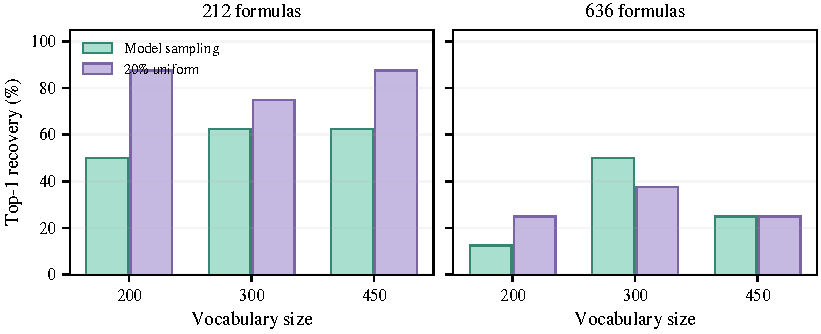
\includegraphics[width=\linewidth]{figures/vocab_sampling.pdf}\caption{种子525下的词表大小与随机生成对照。不混入随机分布时按模型概率采样；20\% uniform表示混入均匀随机token。}\label{fig:vocab_sampling}\end{figure}






\FloatBarrier
\section{简单到复杂的泛化实验}\label{app:generalization}
公式复杂度为
\begin{equation*}
 K=0.40h(L/60)+0.20h(C_{\rm cmd}/6)+0.15h(D/3)+0.15h(S/18)+0.10h(O/12),\quad h(v)=\min(v,2),
\end{equation*}
五个分量按公式的LaTeX源码计算。以\verb|(\Delta{u})=0|为例：
\begin{itemize}\setlength{\itemsep}{3pt}\setlength{\parsep}{0pt}
\item \textbf{词法单元数$L$。}将源码拆为完整LaTeX命令、完整数字串及其他单字符，空白不计；重复出现的单元分别计数。本例依次为\verb|(|、\verb|\Delta|、\verb|{|、\verb|u|、\verb|}|、\verb|)|、\verb|=|、\verb|0|，因此$L=8$。
\item \textbf{LaTeX命令种类数$C_{\rm cmd}$。}统计反斜杠后接英文字母的不同命令，同一命令重复出现只算一种。本例只有\verb|\Delta|，因此$C_{\rm cmd}=1$。
\item \textbf{最大括号嵌套深度$D$。}圆括号、花括号和方括号每打开一层，深度加1，闭合后减1，取全过程最大值。本例外层\verb|(...)|中嵌套\verb|{u}|，因此$D=2$。
\item \textbf{非括号符号种类数$S$。}去掉六种括号字符后，统计不同词法单元的种数，命令和数字串各作为一个单元。本例剩下\verb|\Delta|、\verb|u|、\verb|=|、\verb|0|，因此$S=4$。
\item \textbf{运算符数$O$。}逐次统计\verb|+ - * / = < > ^ _|及\verb|\sum|、\verb|\prod|、\verb|\int|、\verb|\partial|、\verb|\nabla|、\verb|\frac|、\verb|\sqrt|的出现次数。本例只有\verb|=|计入，\verb|\Delta|不在该计数集合中，因此$O=1$。
\end{itemize}
代入$(L,C_{\rm cmd},D,S,O)=(8,1,2,4,1)$，得到$K=0.2283$。

按复杂度排序，最低30\%为简单公式（191条），最高30\%为复杂公式（190条），其余255条为一般公式；实验使用训练划分中的173条简单公式训练，以验证和测试划分中的27条和21条复杂公式评价。AST-BPE的测试压缩率为5.426和6.138，高于通用分词器的1.758--1.834，并保持完整命令。
\begin{table}[H]
\caption{简单公式训练、复杂公式测试，测试集21条。指标与表\ref{tab:upstream}相同。}\label{tab:generalization}
\centering\small\begin{tabular*}{\linewidth}{@{\extracolsep{\fill}}lrrrr@{}}\toprule
分词器 & 压缩率$\uparrow$ & 命令完整率(\%) & 数字完整率(\%) & 使用率(\%)\\\midrule
AST-BPE 300 & 5.426 & \textbf{100.0} & 100.0 & 21.6\\
AST-BPE 450 & \textbf{6.138} & \textbf{100.0} & 100.0 & 16.0\\
Qwen2.5 & 1.834 & 0.0 & 100.0 & --\\
Llama 3 & 1.834 & 0.0 & 100.0 & --\\
\texttt{o200k\_base} & 1.758 & 0.0 & 100.0 & --\\
\bottomrule\end{tabular*}
\end{table}


\clearpage
\section{不同语料与词表大小下的token频率分布}\label{app:token_frequency}
\begin{figure}[H]
\centering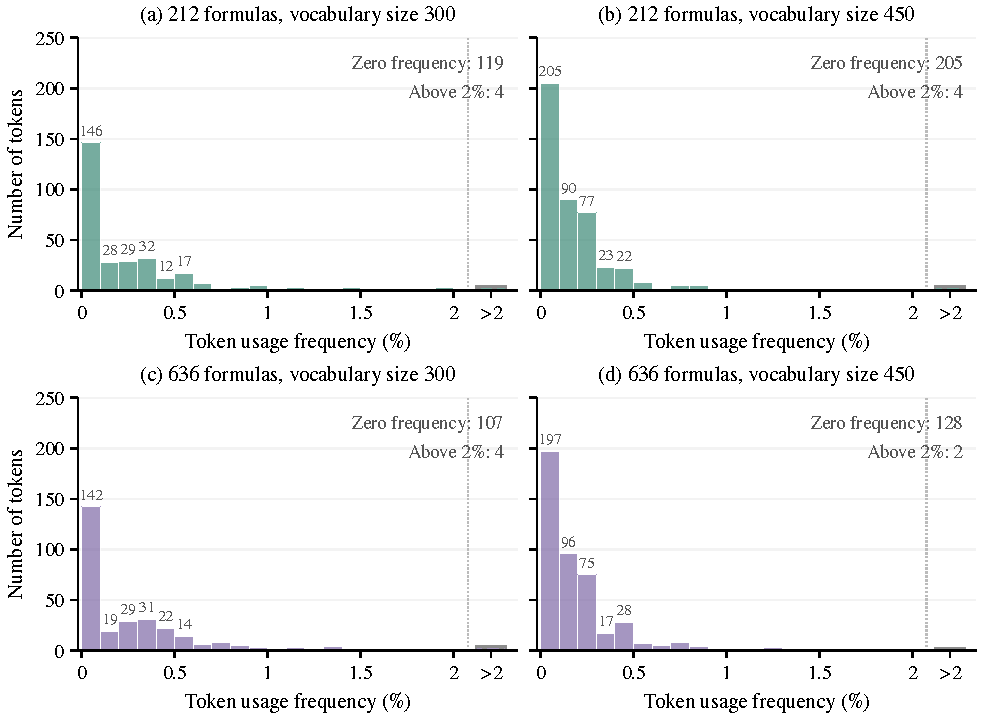
\includegraphics[width=\linewidth]{figures/token_id_frequency.pdf}
\caption{token使用率直方图。横轴为各token的出现次数占比，纵轴为对应区间的token个数；柱宽0.1个百分点，零频率计入首箱。}\label{fig:token_frequency}
\end{figure}

可以发现，四组词表中的token主要集中在低使用率区间，只有少量token的使用率超过2\%，分布呈右偏形态。零频率token在小语料的两种词表中分别有119和205个，在大语料中分别有107和128个。

同一词表大小下，大语料使用了更多种token：两种词表分别从178、242种增至190、319种。词表大小从300增至450时，小语料的零频率token比例从40.1\%升至45.9\%，大语料则从36.0\%降至28.6\%。

\end{document}
